% Traductions et équivalences

\begin{frame}[c]
  \frametitle{Équivalences entre les sémantiques de Frappes de Processus}

% \begin{center}
% 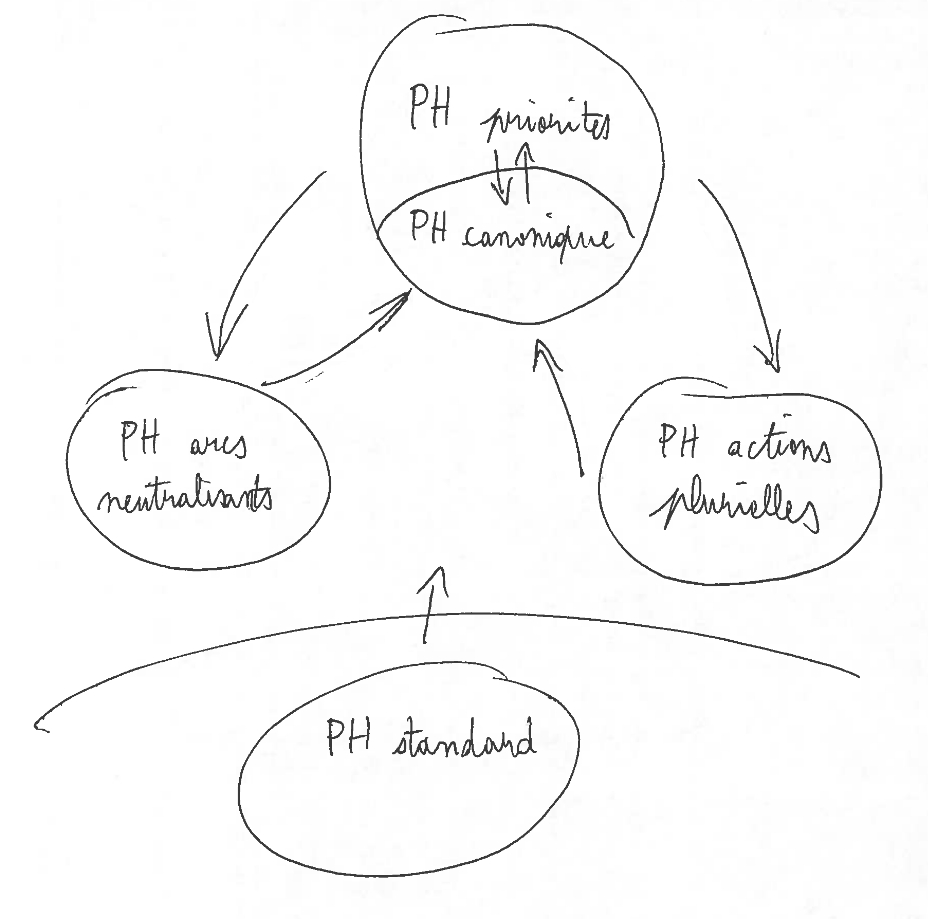
\includegraphics[height=.5\textheight]{figs/PH1.png}
% \end{center}

\setbeamercovered{transparent}

\begin{center}
\scalebox{.8}{
\begin{tikzpicture}
  \path[use as bounding box] (-5.2,-4) rectangle (5.2,3.5);
  \planPHstandard
  \planPHp
  \planPHan
  \planPHmult
  \planPHcanonique
  
  \uncover<2->{
    \path[draw, very thick, bend right=10] (-0.2,2.2) edge[->] (-.2,1.6);
    \path[draw, very thick, bend left=10] (0.2,2.2) edge[<-] (.2,1.6);
  }
  
  \uncover<3->{
    \path[draw, very thick, bend right=10] (-2,1.8) edge[->] (-3,.5);
    \path[draw, very thick, bend right=10] (-2,0) edge[->] (-1,1.1);
  }
  
  \uncover<4->{
    \path[draw, very thick, bend left=10] (2,1.8) edge[<-] (3,.5);
    \path[draw, very thick, bend left=10] (2,0) edge[<-] (1,1.1);
  }
  
  \uncover<5->{
    \planPHstandardligne
    \path[draw, very thick, bend left=10] (0,-1.9) edge[->] (0,-.8);
  }
\end{tikzpicture}
}
\end{center}

Toutes les sémantiques développées sont équivalentes
\begin{itemize}
  \item Importantes possibilités d'expression
  \item Au prix d'une complexité parfois exponentielle
  \item Toujours traduisibles en forme canonique
\end{itemize}

\end{frame}



\setbeamercovered{transparent}

\begin{frame}[c]
  \frametitle{Traductions depuis et vers d'autres modèles discrets}

% \begin{center}
% \hspace*{-1cm}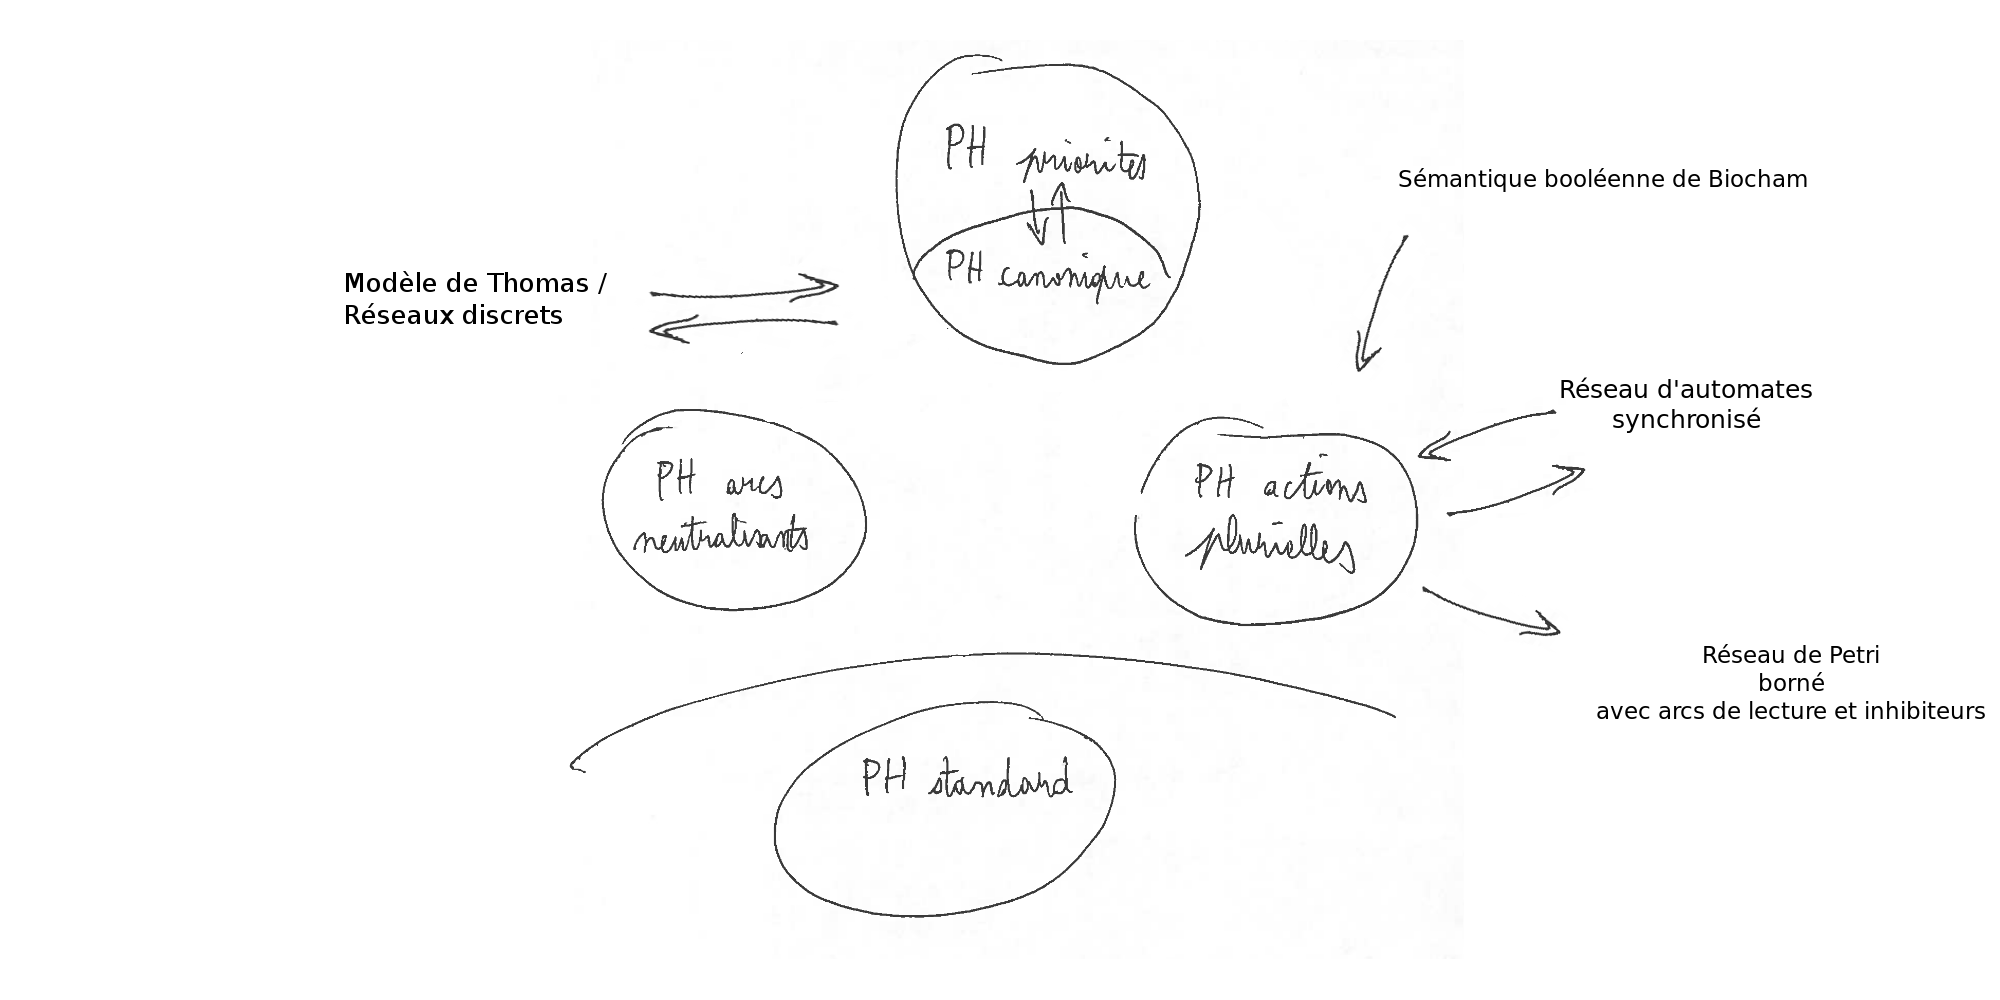
\includegraphics[height=.6\textheight]{figs/PH2.png}
% \end{center}

\begin{center}
\scalebox{.7}{
\begin{tikzpicture}
  \path[use as bounding box] (-5.2,-4) rectangle (5.2,3.5);
  \planPHstandard
  \planPHp
  \planPHan
  \planPHmult
  \planPHcanonique
  \planPHstandardligne
  
  \uncover<2->{
    \draw[thick, draw=black, fill=gray!10] (-4.5,2.5) ellipse (1.4 and .6)
      node[text width=4cm, align=center] {\small Modèle de Thomas\\Réseaux discrets};
    \path[draw, very thick, bend left=5] (-3.3,2.5) edge[->] (-1.5,1.4);
    \path[draw, very thick, bend right=5] (-3.4,2.3) edge[<-] (-1.6,1.2);
  }
  
  \uncover<3->{
    \draw[thick, draw=black, fill=gray!10] (6,2) ellipse (1.2 and .5)
      node[text width=4cm, align=center] {\small Automates\\synchronisés};
    \path[draw, very thick, bend left=5] (6,1.6) edge[->] (4.7,0.4);
    \path[draw, very thick, bend right=5] (5.7,1.7) edge[<-] (4.4,0.5);
  }
  
  \uncover<4->{
    \draw[thick, draw=black, fill=gray!10] (4.2,3.2) ellipse (1.7 and .5)
      node[text width=4cm, align=center] {\small Sémantique booléenne\\de Biocham};
    \path[draw, very thick, bend right=5] (4.2,2.8) edge[->] (3.7,0.6);
  }
  
  \uncover<5->{
    \draw[thick, draw=black, fill=gray!10] (6,-1.7) ellipse (1.7 and .5)
      node[text width=4cm, align=center] {\small Réseaux de Petri bornés\\avec arcs inhibiteurs};
    \path[draw, very thick, bend right=5] (5.7,-1.4) edge[<-] (4.2,-.6);
  }
\end{tikzpicture}
}
\end{center}

\begin{itemize}
  \item Équivalence avec les réseaux discrets / le modèle de Thomas
  \item Équivalence avec les réseaux d'automates synchronisés
  \item Traduction vers les réseaux de Petri (bornés) avec arcs inhibiteurs
  \item Traduction depuis la sémantique booléenne de Biocham.
\end{itemize}

\end{frame}

\setbeamercovered{invisible}
